\documentclass[11pt]{article}

\usepackage[german]{babel} % for PCs
\usepackage[latin1]{inputenc} % for PCs
\usepackage{graphicx}
\usepackage{hyperref}

\oddsidemargin=0in
\evensidemargin=0in
\topmargin=0in
\textwidth=6in
\textheight=8.5in
\pagestyle{plain}


%\nofiles
\begin{document}
\title{\bf Curriculum Vitae}
\author {Ulderico Fugacci}


\date{}
\maketitle


\noindent
{\Large\bf Personal}
\noindent\\

\begin{minipage}{.70\textwidth}

\vspace*{1ex}

Nationality: Italian\\
Sex: Male\\
Date of birth: August 31, 1988\\
Place of birth: Genova, GE, Italy\\

%\begin{itemize}
%\item[ ] Nationality: Italian
%\item[ ] Sex: Male
%\item[ ] Date of birth: August 31, 1988
%\item[ ] Place of birth: Genova, GE, Italy
%\end{itemize}


%\noindent
%{\Large\bf Contacts:}
%\noindent

\vspace*{1ex}

Mobile: (+39) 347 4966799\\
% Mobile: (+39) 347 4966799 \mbox{   } - \mbox{   } (+49) 0173 4763771\\
Email: \href{mailto:ulderico.fugacci@gmail.com}{ulderico.fugacci@gmail.com}\\
Web page: \href{https://fugacci.github.io/home/}{https://fugacci.github.io/home/}\\
% Web page: \href{http://www.umiacs.umd.edu/~fugacci/}{http://www.umiacs.umd.edu/~fugacci/}\\


      \end{minipage}
 \begin{minipage}{.30\textwidth}
\centering
\vspace{-14px}
      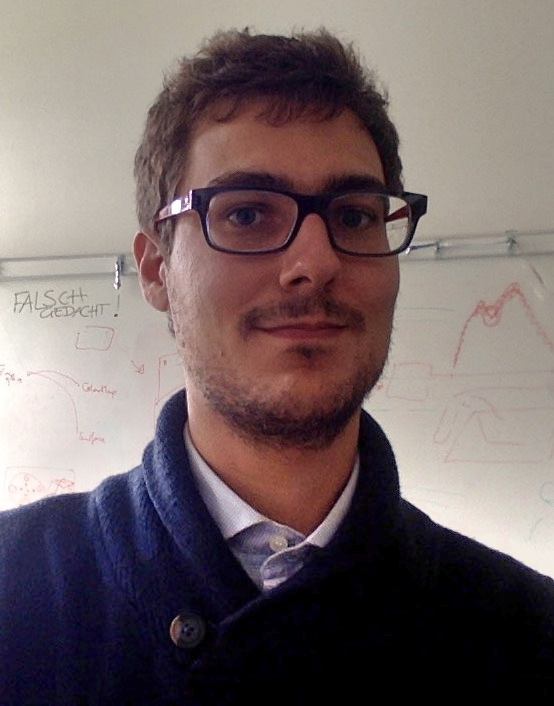
\includegraphics[width=.63\textwidth]{PhotoCV}
      \end{minipage}\\


\noindent
{\Large\bf Education}
\noindent

\begin{itemize}

\item {\bf B.Sc. (Mathematics).} University of Genova, Department of Mathematics. \\Thesis: {\em Ideals of the Ring of Formal Power Series}. \\Advisor: Prof. M. E. Rossi. (September 2010)

\item {\bf M.Sc. (Mathematics).} University of Genova, Department of Mathematics. \\Thesis: {\em Constructive Methods to Compute Simplicial Homology}. \\Advisors: Prof. M. E. Rossi, Prof. L. De Floriani. (July 2012)

\item {\bf Ph.D. (Computer Science).} University of Genova, Department of Computer Science, Bioinformatics, Robotics and Systems Engineering. \\Thesis: {\em Topological Data Analysis through Homology and Discrete Morse Theory}. \\Advisors: Prof. L. De Floriani, Prof. M. E. Rossi. (May 2016)
\end{itemize}




%%%%%%%%%%%%%%%%%%%%%%%%%%%%%%%%%%%%%%%%
\vspace*{2.5ex}

\noindent
{\Large\bf Employments}

\begin{itemize}

\item {\bf July 2020 - Present.} Researcher (III level) at Istituto di Matematica Applicata e Tecnologie Informatiche (IMATI) ``Enrico Magenes'', CNR (National Research Council), Genova, Italy.

\item {\bf July 2019 - June 2020.} Post-doctoral fellow at Department of Mathematical Sciences
% (funded by the Italian MIUR Award ``Dipartimento di Eccellenza 2018-2022'')
and Collaborator of SmartData@PoliTO center for Big Data and Machine Learning technologies, Polytechnic University of Torino, Italy.

\item {\bf November 2017 - June 2019.} Post-doctoral fellow, Institute of Geometry, Graz University of Technology, Austria.

\item {\bf November 2016 - October 2017.} Post-doctoral fellow, Department of Computer Science, Kaiserslautern University of Technology, Germany.

% \item March 2016 - October 2016. Post-doctoral fellow (March - August) and Collaborator (September - October), Department of Computer Science, University of Maryland at College Park, USA.

\item {\bf March 2016 - October 2016.} Post-doctoral fellow, Department of Computer Science, University of Maryland at College Park, MD, USA.

\item {\bf April 2016 - May 2016.} External collaborator, Department of Mathematics, University of Genova, Italy.

\item {\bf January 2013 - February 2016.} Research assistant, Department of Computer Science, Bioinformatics, Robotics and Systems Engineering, University of Genova, Italy.

\end{itemize}


%%%%%%%%%%%%%%%%%%%%%%%%%%%%%%%%%%

\vspace*{3ex}

\noindent
{\Large\bf Research Interests}

\begin{itemize}

\item Topological Data Analysis and Visualization
\item Computational Topology and Geometry
\item Homology, Persistent and Multi-Parameter Persistent Homology
\item Discrete Morse Theory
\item Complex Network Analysis
\item Algorithms and Spatial Data Structures
\item Combinatorics and Commutative Algebra

\end {itemize}




%%%%%%%%%%%%%%%%%%%%%%%%%%%%%%%%%%%%%%%%%%%%%%%%%%%


\vspace*{3ex}
\noindent
{\Large\bf Publications}

%%%%%%%%%%%%%%%%%%%%%%%%%%%%%%%%%%
\vspace*{1.5ex}

\noindent
{\bf Papers in Refereed Journals}

\begin{enumerate}

\item {\bf U. Fugacci, C. Landi, H. Varl{\i}.} {\em Critical Sets of PL and Discrete Morse Theory: a Correspondence}, In Computers \& Graphics, vol. 90, pages 43-50, 2020.

\item {\bf R. Fellegara, F. Iuricich, L. De Floriani, U. Fugacci.} {\em Efficient Homology-Preserving Simplification of High-Dimensional Simplicial Shapes}. In Computer Graphics Forum, vol. 39(1), pages 244-259, 2020.

\item {\bf D. Bolognini, U. Fugacci.} {\em Betti Splittings from a Topological Point of View}. In Journal of Algebra and Its Applications, vol. 19(6), page 2050116, 2020.

\item {\bf R. Corbet, U. Fugacci, M. Kerber, C. Landi, B. Wang.} {\em A Kernel for Multi-Parameter Persistent Homology}. In Computers and Graphics, vol. 2, page 100005, 2019.

\item {\bf U. Fugacci, F. Iuricich, L. De Floriani.} {\em Computing Discrete Morse Complexes from Simplicial Complexes}, In Graphical Models, vol. 103, page 101023, 2019.

\item {\bf B. Rieck, U. Fugacci, J. Lukasczyk, H. Leitte.} {\em Clique Community Persistence: A Topological Visual Analysis Approach for Complex Networks}. In IEEE Transactions on Visualization and Computer Graphics, vol. 24(1), pages 822-831, 2018.

\item {\bf F. Iuricich, U. Fugacci, L. De Floriani.} {\em Topologically-Consistent Simplification of Discrete Morse Complex}. In Computers and Graphics, vol. 51, pages 157-166, 2015. %Awarded with an honorable mention

\item {\bf L. De Floriani, U. Fugacci, F. Iuricich, P. Magillo.} {\em Morse Complexes for Shape Segmentation and Homological Analysis: Discrete Models and Algorithms}. In Computer Graphics Forum, vol. 34(2), pages 761-785, 2015.

\item {\bf L. {\v C}omi{\' c}, L. De Floriani, F. Iuricich, U. Fugacci.} {\em Topological Modifications and Hierarchical Representation of Cell Complexes in Arbitrary Dimensions}. In Computer Vision and Image Understanding, vol. 121, pages 2-12, 2014.

\end{enumerate}
%%%%%%%%%%%%%%%%%%%%%%%%%%%%%%%%%%
\vspace*{1ex}

\noindent
{\bf Refereed Book Chapters}

\begin{enumerate}

\item {\bf L. De Floriani, U. Fugacci, F. Iuricich.} {\em Homological Shape Analysis through Discrete Morse Theory}.  M. Breu{\ss}, A. Bruckstein, P. Maragos, S. Wuhrer (Eds.). In Perspectives in Shape Analysis. Springer International Publishing, pages 187-209, 2016.

\end{enumerate}
%%%%%%%%%%%%%%%%%%%%%%%%%%%%%%%%%%
\vspace*{3ex}

\noindent
{\bf Refereed Conference Papers}
\begin{enumerate}

\item {\bf U. Fugacci, M. Kerber, H. Manet.} {\em Topology-Preserving Terrain Simplification}. In 28th ACM SIGSPATIAL International Conference on Advances in Geographic Information Systems, 2020.

\item {\bf F. Della Santa, M. Ferrara, M. Bilardo, A. De Gregorio, U. Fugacci, A. Mastropietro, E. Fabrizio, F. Vaccarino.} {\em Application of Deep Learning to Design Renewable Energy Systems for a Zero Energy Multifamily Building}. In 15th Conference on Sustainable Development of Energy, Water and Environment Systems, 2020.

\item {\bf U. Fugacci, M. Kerber.} {\em Chunk Reduction for Multi-Parameter Persistent Homology}. In 39th International Symposium on Computational Geometry, 2019.

\item {\bf R. Fellegara, U. Fugacci, F. Iuricich, L. De Floriani.} {\em Analysis of Geolocalized Social Networks based on Simplicial Complexes}. In 9th ACM SIGSPATIAL International Workshop on Location-Based Social Networks, 2016.

\item {\bf U. Fugacci, S. Scaramuccia, F. Iuricich, L. De Floriani.} {\em Persistent Homology: a Step-by-Step Introduction for Newcomers}. G. Pintore and F. Stanco (Eds.). In Smart Tools and Apps for Graphics - Eurographics Italian Chapter Conference, The Eurographics Association, 2016.

\item {\bf U. Fugacci, F. Iuricich, L. De Floriani.} {\em Efficient Computation of Simplicial Homology through Acyclic Matching}. In 16th International Symposium on Symbolic and Numeric Algorithms for Scientific Computing, pages 587-593, 2014.

\end{enumerate}
%%%%%%%%%%%%%%%%%%%%%%%%%%%%%%%%%%
\vspace*{1ex}

\noindent
{\bf Communications at International Conferences and Workshops}
\begin{enumerate}

\item {\bf U. Fugacci, M. Kerber, H. Manet.} {\em Topology-Aware Terrain Simplification}:
\begin{enumerate}
  \item Poster, Algebraic Topology: Methods, Computation and Science, 2018.
  \item Extended Abstract, Computational Geometry: Young Researchers Forum, 2018.
\end{enumerate}

\item {\bf R. Corbet, U. Fugacci, M. Kerber, C. Landi, B. Wang.} {\em A Kernel for Multi-Parameter Persistent Homology}:
\begin{enumerate}
  \item Poster, Algebraic Topology: Methods, Computation and Science, 2018.
  \item Extended Abstract, Computational Geometry: Young Researchers Forum, 2018.
\end{enumerate}

% \item {\bf L. {\v C}omi{\' c}, L. De Floriani, F.Iuricich, U. Fugacci.} {\em A Hierarchical Approach to Topological Shape Analysis}, Poster, XXXXXXX, 201X.

\end{enumerate}
%%%%%%%%%%%%%%%%%%%%%%%%%%%%%%%%%%
\vspace*{1ex}

\noindent
{\bf On-Going Papers}
\begin{enumerate}

\item {\bf A. De Gregorio, U. Fugacci, F. M\'emoli, F. Vaccarino.} {\em On the Notion of Weak Isometry for Finite Metric Spaces}. Under submission, preprint available at arXiv.org.

\item {\bf M. Guerra, A. De Gregorio, U. Fugacci, G. Petri, F. Vaccarino.} {\em Homological Scaffold via Minimal Homology Bases}. Under submission, preprint available at arXiv.org.

\item {\bf U. Fugacci.} {\em Persistence-Based Kernels for Data Classification}. Under submission.

\item {\bf M. Ferrara, F. Della Santa, M. Bilardo, A. De Gregorio, U. Fugacci, A. Mastropietro, F. Vaccarino, E. Fabrizio.} {\em Deep Learning-Based Optimization Methods for Integrated Design of Zero Energy Buildings}. Under submission.

% \item {\bf M. Bilardo, A. De Gregorio, F. Della Santa, E. Fabrizio, M. Ferrara, U. Fugacci, A. Mastropietro, F. Vaccarino.} {\em Application of Deep Learning to Design Renewable Energy Systems for a Zero Energy Multifamily Building}, under submission.

% \item {\bf U. Fugacci, F. Iuricich, S. Scaramuccia, L. De Floriani.} {\em Mult-Parameter Persistent Homology for Shape Analysis}, in preparation.
%
% \item Topological Signature of DNN
%
% \item Eulero & co.
%
% \item Feature-Based Persistence
%
% \item Capitolo Ciccio MUltipersistenza

\end{enumerate}


\vspace*{2.5ex}
\noindent
{\Large\bf Awards}
\begin{itemize}
\item SMI 2015 - {\bf Honorable Mention}, {\em Topologically-Consistent Simplification of Discrete Morse Complex} (joint work with F. Iuricich and L. De Floriani).
%\item SMI 2015 - Honorable Mention for the presentation of the paper {\em Topologically-Consistent Simplification of Discrete Morse Complex} (joint work with F. Iuricich, L. De Floriani)
\item {\bf 2016 Best Ph.D. Thesis in Computer Science}, University of Genova.
\item SMI 2019 - {\bf Best Paper}, {\em A Kernel for Multi-Parameter Persistent Homology} (joint work with R. Corbet, M. Kerber, C. Landi, B. Wang).
\end{itemize}


\vspace*{2.5ex}
\noindent
{\Large\bf Participations in Research Projects}
\begin{itemize}
\item Mesh-Based Representation and Topological Analysis of Static and Time-varying 3D Scalar Fields and 4D Shapes (NSF project IIS-1116747).
\item Commutative Algebra and Applications (project CARIGE).
\item Algorithms for Topological Data Analysis (Austrian Science Fund (FWF) - grant P29984-N35).
\item Italian MIUR Award ``Dipartimento di Eccellenza 2018-2022'' Disma-PoliTO - CUP: E11G18000350001
\item ELBA, Establishment of Training and Research Centers and Courses Development on Intelligent Big Data Analysis in Central Asia.
\end{itemize}

% \vspace*{1ex}
% \noindent
% {\bf Memberships}
% \begin{itemize}
% \item IEEE Member
% \end{itemize}


%%%%%%%%%%%%%%%%%%%%%%%%%%%%%%%%%%%%%%%%%%%%%%%%%%%%%%

\vspace*{2.5ex}
\noindent
{\Large\bf Professional Service}

\vspace*{1.5ex}
\noindent
{\bf Reviewing Activity}
\begin{itemize}
  \item ACM Transactions on Spatial Algorithms and Systems (TSAS), 2017.
  \item 34th International Symposium on Computational Geometry, SoCG 2018.
  \item 26th Annual European Symposium on Algorithms, ESA 2018.
  \item 19th International Workshop on Combinatorial Image Analysis, IWCIA 2018.
  \item International Conference on Algebra and Related Topics, ICART 2018 (Special issue of the Journal Algebra Colloquium).
  \item Proceedings of the Royal Society A (RSPA), 2019.
  \item Journal of Computational Geometry (JoCG), 2019.
  \item Statistics in Transition New Series (SiT), 2019.
  \item 36th International Symposium on Computational Geometry, SoCG 2020.
  \item International Workshop on Combinatorial Image Analysis, IWCIA 2020.
  \item Graphical Models (GMOD), 2020.
\end{itemize}

\vspace*{1ex}
\noindent
{\bf Organization of Scientific Events}
\begin{itemize}
\item Local organizer for the School ``Homology: Theoretical and
Computational Aspects'',  International School, jointly organized by the Department of Computer Science, Bioinformatics, Robotics and Systems Engineering and by the Department of Mathematics of the University Genova, February 2015.
\item Organizer of the session on ``Geometric Aspects of Applied Topology'' at the Joint Meeting of UMI-SIMAI-PTM, Wroc\l{}aw, Poland, September 2018.
\item Organizer of the ``6th SmartData@PoliTO Workshop'' at Castello del Valentino, Torino, Italy, January 2020.
% \item Organizer of MAIn 2020 (Mathematics for Artificial Intelligence)???
\end{itemize}

\vspace*{2.5ex}
\noindent
{\Large\bf Courses and Talks in Conferences and International Schools}

\vspace*{1.5ex}
\noindent
{\bf Courses and Seminars in International Schools}

\begin{itemize}
  \item Invited lecturer of the course {\em Persistent Homology: from Theory to Applications} (3 lectures + 1 lab session) given at ``Persistent Homology'' Summer School, Rabat, Morocco, July 2017.
\end{itemize}

\vspace*{1ex}
\noindent
{\bf Presentations and Talks in International Venues}

\begin{itemize}

\item {\em Efficient Computation of Simplicial Homology through Acyclic Matching}, presented at CTIC 2014, Computational Topology in Image Context at SYNASC 2014, West University of Timisoara, Romania, September 2014.

\item {\em Topologically-Consistent Simplification of Discrete Morse Complex}, presented at SMI 2015, Shape Modeling International, Lille 1 University, France, June 2015.

\item {\em Efficient Computation of Persistence Homology through Discrete Morse Theory}, presented at CAT-School 2015, Computational Algebraic Topology, University of Oxford, UK, September 2015.

\item {\em Topological Data Analysis through Homology and Discrete Morse Theory}, presented at Kaiserslautern University of Technology, Germany, May 2016.

\item {\em Persistent Homology: a Step-by-Step Introduction for Newcomers}, presented at STAG 2016, Smart Tools and Apps for Graphics, Genova, Italy, October 2016.

\item {\em Homology and Discrete Morse Theory in Topological Data Analysis}, presented at Graz University of Technology, Austria, February 2017.

\item {\em Clique Community Persistence: A Topological Visual Analysis Approach for Complex Networks}, presented at SciVis, IEEE VIS 2017, Phoenix, AZ, USA, October 2017.

\item {\em Topology-Aware Terrain Simplification}, presented at YRF - SoCG 2018, 34th International Symposium on Computational Geometry, Budapest, Hungary, June 2018.

\item {\em A Kernel for Multi-Parameter Persistent Homology}, poster presented at ATMCS8, Algebraic Topology: Methods, Computation and Science, Klosterneuburg, Austria, June 2018.

\item {\em Topology-Based Tools for Data Classification}, presented at Polytechnic University of Torino, Italy, December 2018.

\item {\em Limits and New Perspectives in Topological Data Analysis}, presented at Paris Diderot University, France, January 2019.

\item {\em Topological Data Analysis: Application-Driven Strategies for Compactness and Efficiency}, presented at SmartData@PoliTO - Polytechnic University of Torino, Italy, April 2019.

\item {\em Chunk Reduction for Multi-Parameter Persistent Homology}, presented at SoCG 2019, 35th International Symposium on Computational Geometry, Portland, OR, USA, June 2019.

\item {\em Topological Tools in Data Analysis}, presented at 5th SmartData@PoliTO Workshop, Barolo, Italy, September 2019.

\item {\em Persistence-Based Kernels for Data Classification}, presented at Complex Simplex: Topological and Network Data Science Workshop, Torino, Italy, October 2019.

\item {\em On the encoding of large, high-dimensional, and unorganized datasets}, presented at 6th SmartData@PoliTO Workshop, Torino, Italy, January 2020.

% \item {\em Topology of Data}, presented at Advisory Board of the project ``Dipartimento di Eccellenza 2018-2022", Torino, Italy, February 2020.

\item {\em Critical Sets of PL and Discrete Morse Theory: a Correspondence}, presented at SMI 2020, Shape Modeling International, Strasbourg, France, June 2020.
% coronavirus

% CAMBIA TITOLO? E' UGUALE A UNO DEI PRECEDENTI. \item {\em Persistence-Based Kernels for Data Classification}, presented at SIS 2020, 50th Scientific Meeting of the Italian Statistical Society, Pisa, Italy, June 2020.

\item {\em Topological tools for Network Description}, keynote speech at TopoNets 2020 - Networks beyond pairwise interactions, Satellite @ NetSci 2020, Rome, Italy, September 2020.
% coronavirus

% \item {\em Topology-Preserving Terrain Simplification}, presented at 28th ACM SIGSPATIAL International Conference on Advances in Geographic Information Systems, Seattle, WA, USA, November 2020.
% % coronavirus

\end{itemize}

\vspace*{2.5ex}
\noindent
{\Large\bf Participations in Conferences, Workshops and Schools}
\vspace*{0.5ex}
\begin{itemize}
\item[ ]{\bf 2011}
\begin{itemize}
\item{MONICA 2011, MONomial Ideals, Computations and Applications, Castro Urdiales, Spain. (July 2011)}
\end{itemize}
\vspace*{0.2ex}
\item[ ]{\bf 2012}
\begin{itemize}
\item{VisMac 2012, School on Machine Vision, Genova, Italy. (October 2012)}
\end{itemize}
\vspace*{0.2ex}
\item[ ]{\bf 2013}
\begin{itemize}
\item{BiSS 2013, Bertinoro international Spring School, Bertinoro, Italy. (March 2013)}
\item{EACA's Second International School On Computer Algebra and Applications, Valladolid, Spain. (June 2013)}
\item{ACAT's Summer School on Computational Topology and Topological Data Analysis, Ljubljana, Slovenia. (July 2013)}
\item{INdAM Meeting CoMeTA 2013, Combinatorial Methods in Topology and Algebra, Cortona, Italy. (September 2013)}
\end{itemize}
\vspace*{0.2ex}
\item[ ]{\bf 2014}
\begin{itemize}
\item{IMA Annual Program Year Workshop, Topology and Geometry of Networks and Discrete Metric Spaces, Minneapolis, MN, USA. (April-May 2014)}
\item{VisMac 2014, Summer School on Computer Vision and Pattern Recognition for Homeland Security, Marina di Ascea, Italy. (June 2014)}
\item{SYNASC 2014, International Symposium on Symbolic and Numeric Algorithms for Scientific Computing, Timisoara, Romania. (September 2014)}
\end{itemize}
\vspace*{0.2ex}
\item[ ]{\bf 2015}
\begin{itemize}
\item{HTCA-2015 International School, Homology: Theoretical and Computational Aspects, Genova, Italy. (February 2015)}
\item{SMI 2015, Shape Modeling International, Lille, France. (June 2015)}
\item{CAT-School 2015, Computational Algebraic Topology; ATI scoping workshop, Topological Data Analysis, Oxford, UK. (September 2015)}
\item{Incontro di Algebra Commutativa, Genova, Italy. (October 2015)}
\end{itemize}
\vspace*{0.2ex}
\item[ ]{\bf 2016}
\begin{itemize}
\item{SoCG 2016, 32th International Symposium on Computational Geometry, Boston, MA, USA. (June 2016)}
\item{STAG 2016, Smart Tools and Apps for Graphics, Genova, Italy. (October 2016)}
\end{itemize}
\vspace*{0.2ex}
\item[ ]{\bf 2017}
\begin{itemize}
\item{``Persistent Homology'' Summer School, Rabat, Morocco. (July 2017)}
\item{IEEE VIS 2017, Phoenix, AZ, USA. (October 2017)}
\end{itemize}
\vspace*{0.2ex}
\item[ ]{\bf 2018}
\begin{itemize}
\item{TAGS, Linking Topology to Algebraic Geometry and Statistics, Leipzig, Germany. (February 2018)}
\item{SoCG 2018, 34th International Symposium on Computational Geometry, Budapest, Hungary. (June 2018)}
\item{ATMCS8, Algebraic Topology: Methods, Computation and Science, Klosterneuburg, Austria. (June 2018)}
\item{Joint Meeting of UMI-SIMAI-PTM, Wroc\l{}aw, Poland. (September 2018)}
\end{itemize}
\vspace*{0.2ex}
\item[ ]{\bf 2019}
\begin{itemize}
\item{East Austria Topological Data Analysis Meeting, Graz, Austria. (January 2019)}
\item{SoCG 2019, 35th International Symposium on Computational Geometry, Portland, OR, USA. (June 2019)}
\item{{\"O}MG Conference 2019, Dornbirn, Austria. (September 2019)}
\item{5th SmartData@PoliTO Workshop, Barolo, Italy. (September 2019)}
\item{Complex Simplex: Topological and Network Data Science Workshop, Torino, Italy. (October 2019)}
\end{itemize}
\vspace*{0.2ex}
\item[ ]{\bf 2020}
\begin{itemize}
\item{6th SmartData@PoliTO Workshop, Torino, Italy. (January 2020)}
\item{SMI 2020, Shape Modeling International, Strasbourg, France. (June 2020)}
% coronavirus
% \item{SIS 2020, 50th Scientific Meeting of the Italian Statistical Society, Pisa, Italy. (June 2020)}
\item{SGP 2020, Symposium on Geometry Processing, Utrecht, Netherland. (July 2020)}
% coronavirus
\item{TopoNets 2020 - Networks beyond pairwise interactions, Satellite @ NetSci 2020, Rome, Italy. (September 2020)}
% coronavirus
% \item{ACM SIGSPATIAL 2020, 28th International Conference on Advances in Geographic Information Systems, Seattle, WA, USA. (November 2020)}
% % coronavirus

\end{itemize}
\end{itemize}

\vspace*{2.5ex}
\noindent
{\Large\bf Short Visits}
\begin{itemize}
\item April 2014 and October-December 2014, University of Maryland, MD, USA.
\item April 2016, University of Miami, FL, USA.
\item May 2016, Kaiserslautern University of Technology, Germany.
\item February 2017 and November 2019, Graz University of Technology, Austria.
\item December 2018 and April 2019, Polytechnic University of Torino, Italy.
\item January 2019, Paris Diderot University, France.
\end{itemize}


%%%%%%%%%%%%%%%%%%%%%%%%%%%%%%%%%%%%%%%%%%%%%%%

\vspace*{2.5ex}

\noindent
{\Large\bf Teaching and Advising Activity}

\vspace*{1.5ex}
\noindent
{\bf At University of Genova}

\begin{itemize}
\item Tutor, Elementi di Matematica e Logica, Undergraduate Program in Computer Science, 2011-2012.
\item Guest lecturer, Geometric Modeling, Master Program in Computer Science and Mathematics, 2012-2013.
\item Assistant tutor for Master Thesis in Mathematics by Beatrice Roticiani, advisor Prof. L. De Floriani, September 2013.
\item Lecturer at Mathematics stage for High School students, February 2014.
\item Assistant tutor for Master Thesis in Mathematics by Simone Rubino, advisor Prof. L. De Floriani, February 2014.
\item Tutor for Mathematics and Physics Undergraduate Students, 2013-2014.
\item Guest lecturer, Geometric Modeling, Master Program in Computer Science and Mathematics, 2013-2014.
\item Guest lecturer, Geometric Modeling, Master Program in Computer Science and Mathematics, 2014-2015.
% \item Assistant to the exams, Algorithms and Data Structures, Undergraduate Program in Computer Science, 2014-2015.
\item Assistant tutor for Master Thesis in Mathematics by Lisa Chiang, advisors Dr. F. Giannini and Dr. M. Monti, March 2015.
\item Teaching assistant, Elementi di Matematica e Logica, Undergraduate Program in Computer Science, 2015-2016.
\item Instructor, Topology-Based Data Analysis and Visualization, Ph.D. Program in Computer Science, 2017-2018.
\item Instructor, Geometria e Applicazioni all'Analisi dei Grafi, Scuola Superiore IANUA-ISSUGE, 2020.
\item Instructor, Analisi Matematica I, Undergraduate Program in Electrical Engineering, 2020-2021.
\end{itemize}

\vspace*{1ex}
\noindent
{\bf At Kaiserslautern University of Technology}

\begin{itemize}
  \item Guest lecturer, Computational Geometry, Master Program in Applied Computer Science, 2016-2017.
  \item Guest lecturer, Visual Analytics, Master Program in Applied Computer Science, 2016-2017.
  \item Co-advisor for Master Thesis in Computer Science by Jan St\"{a}rz, co-advised with Prof. H. Leitte, September 2017.
\end{itemize}

\vspace*{1ex}
\noindent
{\bf At Graz University of Technology}

\begin{itemize}
  \item Co-advisor of the Internship of Hugo Manet, April-August 2018.
  \item Instructor, Knots and 3-Manifolds, Master Program in Mathematics, 2018-2019.
\end{itemize}

\vspace*{1ex}
\noindent
{\bf At Polytechnic University of Torino}

\begin{itemize}
  \item Instructor, Computational Linear Algebra for Large Scale Problems, Master Program in Data Science and Engineering and in Mathematical Engineering, 2019-2020.
  \item Instructor, Top Data Analysis, Ph.D. Program in Pure and Applied Mathematics (joint with University of Torino), 2019-2020.
  % \item 2 Training per ELBA
\end{itemize}

%%%%%%%%%%%%%%%%%%%%%%%%%%%%%%%%%%%%%%%

\vspace*{2.5ex}
\noindent
{\Large\bf Languages}

\begin{itemize}
\item Italian, Mother Tongue
\item English, Full Professional Proficiency
\begin{itemize}
  \item First Certificate (March 2007)
\end{itemize}
\item German, Elementary Proficiency
\begin{itemize}
  \item A2.1 GeR (July 2017)
\end{itemize}
\end{itemize}

%%%%%%%%%%%%%%%%%%%%%%%%%%%%%%%%%%%%%%%

% \vspace*{10ex}
% \vspace*{4ex}
\vspace*{8ex}
\noindent
September 21, 2020
%\today

%\vspace{-10 mm}
%\begin{figure}[hb]
%\flushright
%\includegraphics[width=.3 \textwidth]{signature.png}%
%\end{figure}


\end{document}
